\documentclass{article}

\usepackage[margin=1in]{geometry}
\usepackage{graphicx}
\usepackage{amsmath}
\usepackage{amsfonts}
\usepackage{float}
\usepackage{caption}


\author{\begin{tabular}{l@{\hspace{2em}}r}Zachary \textsc{Vogel}& Maurice \textsc{Woods} III\end{tabular}\\[1.5ex]
\begin{tabular}{l@{\hspace{1.5em}}r}Derek \textsc{Reamon} & Mechatronics\end{tabular}
}
\date{\today}
\title{\textbf{\begin{tabular}{c}Grad Project Proposal in MCEN 5115:\\Rotating Inverted Pendulum\end{tabular}}}

\begin{document}
\maketitle


\section*{Introduction}
This is a proposal for the required Graduate Project in Mechatronics and Robotics. Our group will be attempting to build a closed-loop controller for the rotating inverted pendulum seen in figure 1. We want to be able to keep the freely floating rod straight up, $\alpha=0$. We also want to pursue an open loop actuation that will take the pendulum from $\alpha=\pi$ to $\alpha=0$, at which point we will use the closed loop controller.

\begin{figure}[H]
    \centering
    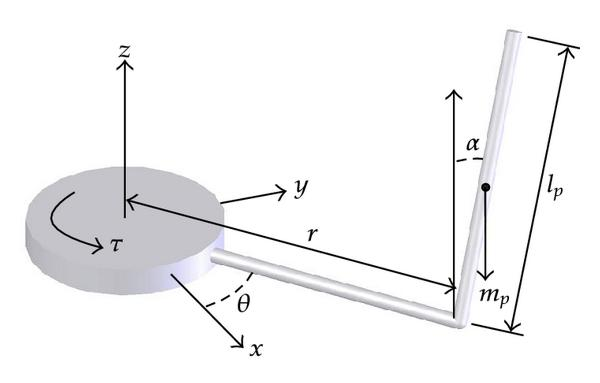
\includegraphics[width=0.6\textwidth]{rotational_pend.jpg}
    \caption{The rotational inverted pendulum we will be building a controller for}
\end{figure}

\section*{Model}
The simplified model considering all torques and forces found on the wikipedia page for Furuta pendulum is quite complex:
\[\begin{array}{c}\ddot{\theta_1}(\hat{J_0}+\hat{J_2}\sin^2(\theta_2))+\ddot{\theta_2}m_2L_1l_2\cos(\theta_2)-m_2L_1l_2\sin(\theta_2)\dot{\theta_2}^2+\dot{\theta_1}\dot{\theta_2}\sin(2\theta_2)\hat{J_2}+b_1\dot{\theta_1}=\tau_1\\\ddot{\theta_1}m_2L_1l_2\cos(\theta_2)+\ddot{\theta_2}\hat{J_2}-\cfrac{1}{2\dot{\theta_1}^2}\sin(2\theta_2)\hat{J_2}+b_2\dot{\theta_2}+gm_2l_2\sin(\theta_2)=\tau_2\end{array}\]
where the following table defines the constants:
\begin{table}[H]
    \centering
    \begin{tabular}{|l|l|l|}
        \hline
        Variable & Equivalent to & Description\\[0.2ex]\hline
        $\alpha$ & $\theta_2+\pi$ & angular position of the pendulum relative to it pointing up\\[0.2ex]\hline
        $\theta_1$ &   & angular position of the rod coming off the motor\\[0.2ex]\hline
        $\theta_2$ & $\alpha-\pi$ & angular position of the pendulum relative to it pointing down\\[0.2ex]\hline
        $l_1$    & & length from motor to center of mass of rod attached to motor\\[0.2ex]\hline
        $l_2$ & & length from end of motor rod to center of mass of pendulum rod\\[0.2ex]\hline
        $L_1$ & & length of rod attached to motor\\[0.2ex]\hline
        $L_2$ & & length of pendulum rod\\[0.2ex]\hline
        $m_1$ & & mass of rod attached to motor\\[0.2ex]\hline
        $m_2$ & & mass of pendulum rod\\[0.2ex]\hline
        $J_1$ & & Inertia tensor about the center of mass of motor rod\\[0.2ex]\hline
        $J_2$ & & Inertia tensor about the center of mass of pendulum rod\\[0.2ex]\hline
        $\tau_1$ & & torque applied to motor rod\\[0.2ex]\hline
        $\tau_2$ & & torque applied to pendulum rod\\[0.2ex]\hline
        $\hat{J_1}$ &$J_1+m_1l_1^2$ & moment of inertia of motor rod about motor pivot\\[0.2ex]\hline
        $\hat{J_2}$ &$J_2+m_2l_2^2$ & moment of inertia of pendulum rod about pivot\\[0.2ex]\hline
        $\hat{J_0}$ &$J_1+m_1l_1^2+m_2L_1^2$ & total moment of inertia exerted on motor rod at equilibrium\\[0.2ex]\hline
    \end{tabular}
\end{table}
Note that equilibrium is when the pendulum rod is pointing downward. Unfortunately, for this project this model is really complex, so we will not be using this explicitly. Instead, we will start with a relatively simple model and add complexity until the system functions appropriately. Thus to begin we will consider the simple dynamics of just an inverted pendulum on a cart:
\[(M+m_2)\ddot{x}-m_2l_2\ddot{\alpha}\cos(\theta)+m_2l_2\dot{\alpha}^2\sin(\alpha)=F\]
\[l_2\ddot{\alpha}-g\sin(\alpha)=\ddot{x}\cos(\alpha)\]
Where M is the mass of the cart and F is the force on the cart. We will rewrite this equation utilizing the torque of the motor, $\tau_1$, as the force. Then this equation can be linearized about the equilibrium position $\alpha=0$ to get a workable equation within some range for $\lvert\alpha\rvert<\epsilon$. If necessary, other terms relating the rotational forces can be added until the model is accurate enough for the device. We will have to do some system identification to get the
values of everything, or pull them from the last people who worked on this.

\section*{Goals \& Control Implementation}
The controller will be implemented on some arm microcontroller that I already own. It will be written in C. The goal is to build a control that keeps the rod pointed upward as long as $\alpha$ stays within some range, $\epsilon$. We would also like to have an open loop control to go from $\alpha=\pi$ to $\alpha=0$. The idea being if the pendulum was not pointed up one could just wait for it to settle than use the open loop control to get it within the range that the closed-loop controller
will work for. The sampling rate will be adjusted on the various encoders to be much higher than the natural frequency of the system, so that we don't have to really consider sampling effects.

\section*{Final Thoughts}
We talked to Quincy who worked on this project previously and she said the encoder was broken on the motor, so we might consider replacing that. We also spoke to a few professors and they seemed to think the above approach would work fairly well. We also know a student who worked on a non-linear controller for a double inverted pendulum last semester who could provide some valuable insight. The final deliverables will be a simulink model, a report, and hopefully a working rotational
pendulum.

\end{document}
